Datensatz: glass

\textbf{Fl\"ache unter ROC Kurve}
\begin{table}[htb]
	\centering
\begin{tabular}{c|c|c|c}
				Regellerner       & \emph{build wind float} & \emph{containers} & \emph{tableware}  \\ \hline
				\emph{J48}			& 0.81 & 0.87 & 0.93  \\ \hline
				\emph{Naive Bayes}  & 0.71 & 0.84 & 0.98  
\end{tabular}
\end{table}

\begin{figure}[htbp]
	\centering
		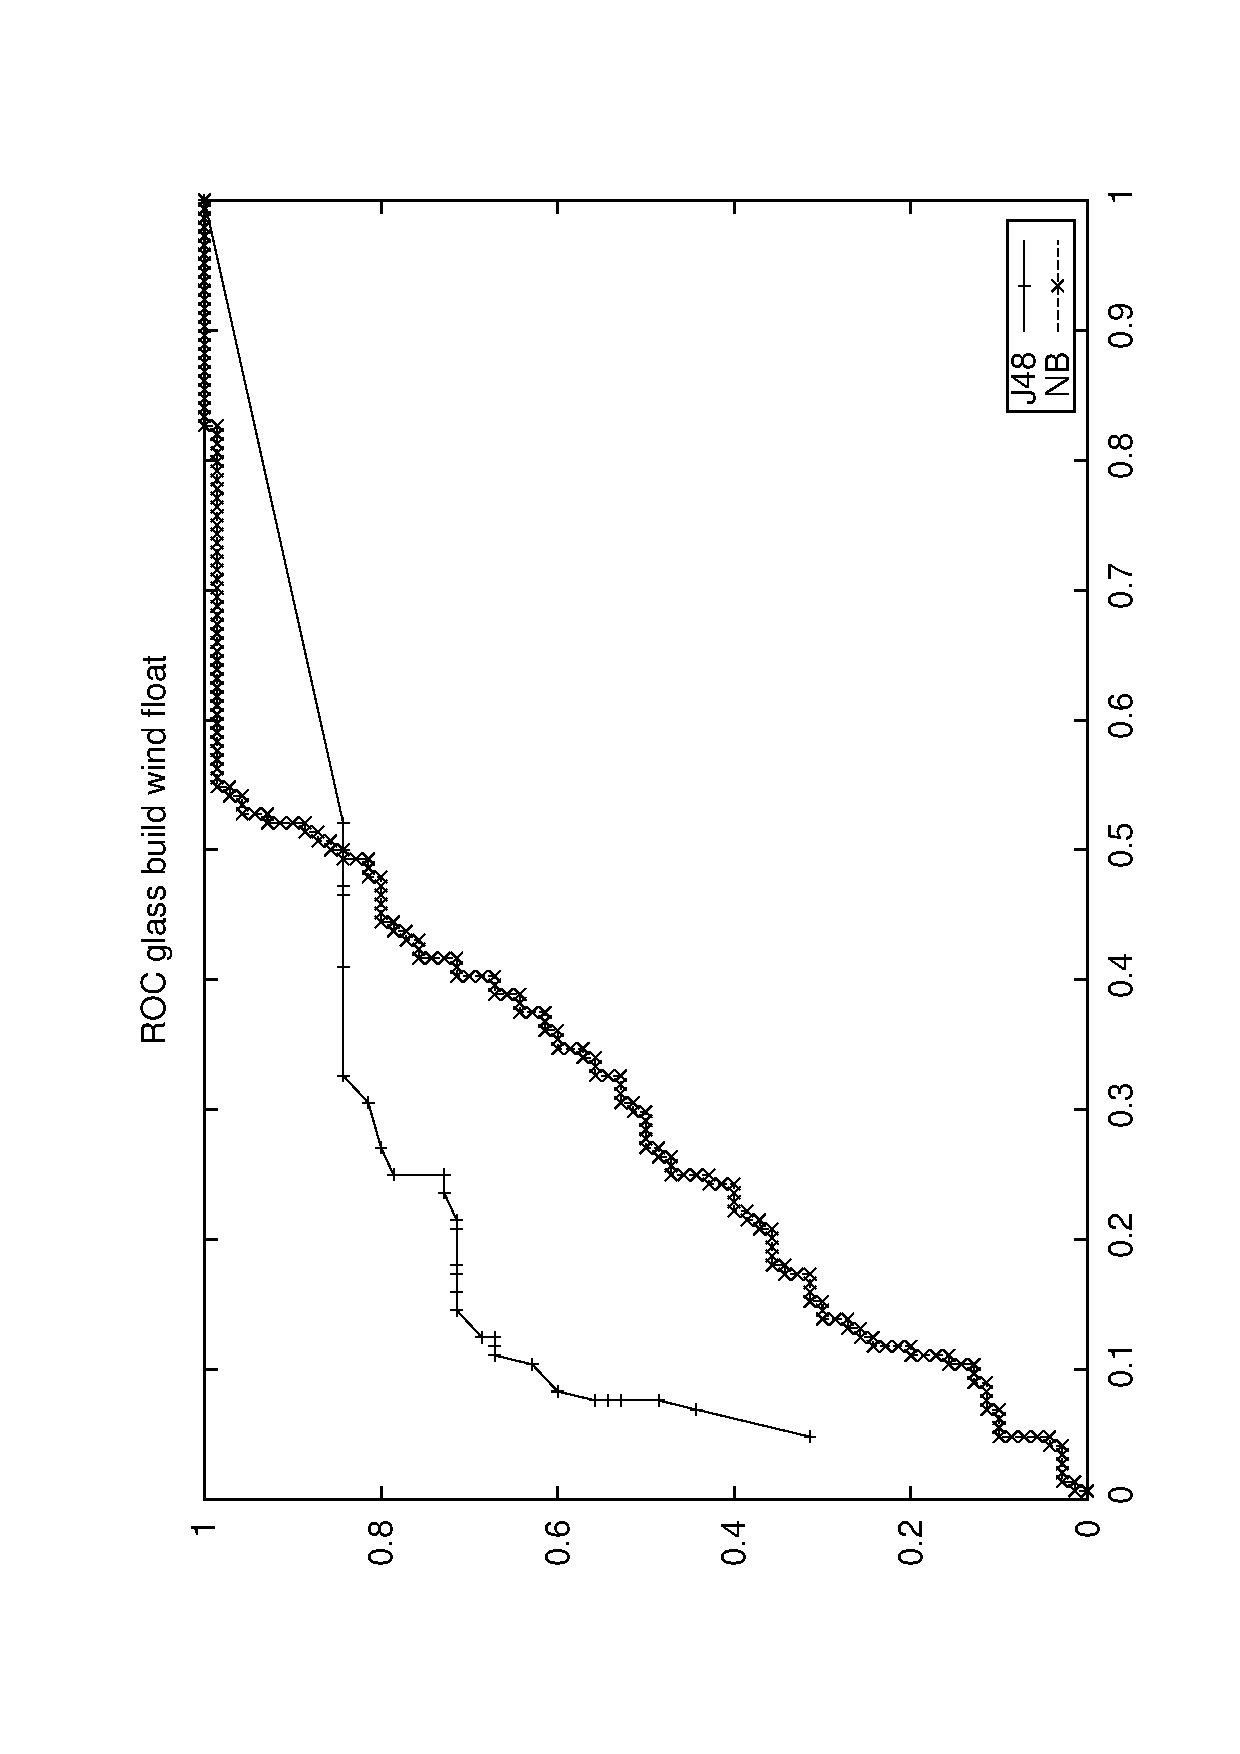
\includegraphics[height=3in]{pics/a3/ROC_glass_build_wind_float.pdf}
	\caption{ROC-Kurve f\"ur \emph{Naive Bayes} und \emph{J48} \"uber das Attribut \emph{build\_wind\_float}}
\end{figure}

\begin{figure}[htbp]
	\centering
		\includegraphics[height=3in]{pics/a3/ROC_glass_containers.pdf}
	\caption{ROC-Kurve f\"ur \emph{Naive Bayes} und \emph{J48} \"uber das Attribut \emph{containers}}
\end{figure}

\begin{figure}[htbp]
	\centering
		\includegraphics[height=3in]{pics/a3/ROC_glass_tableware.pdf}
	\caption{ROC-Kurve f\"ur \emph{Naive Bayes} und \emph{J48} \"uber das Attribut \emph{containers}}
\end{figure}

Bis auf wenige Klassen hat \emph{J48} eine h\"ohere Fl\"ache unter der ROC Kurve.
Anhand der ROC Kurven kann man also sagen, dass f\"ur eine uniforme Klassenverteilung und f\"ur eine Verteilung mit mehr negativen als positiven Beispielen \emph{J48} bessere Ergebnisse liefert. Bei Besonders vielen positiven Beispielen k\"onnte der Naive Bayes Klassifizierer bessere Ergebnisse erzielen.
